\chapter{Recolección de datos de tráfico}
\label{cap:3}

Actualmente existen una variedad de tecnologías para la recolección automática de datos del tráfico. Según Mimbela \cite{mimbela2003summary} podemos dividir estas tecnologías en dos. La primera es la \emph{tecnología in-situ}, que toma los datos del tráfico a través de detectores ubicados a lo largo del camino y que vuelve a dividirse en dos categorías: la intrusiva y la no intrusiva. La segunda, denominada \emph{Floating Car Data} (FCD), es una alternativa para obtener datos del tráfico de gran calidad mediante el uso de vehículos sonda equipados con dispositivos de medición que pueden ser dedicados o no.

\section{Tecnologías in-situ}

Las \emph{tecnologías de detección in-situ} se basan en la recolección de datos mediante dispositivos específicos para este fin que son dispuestos físicamente en los lugares sujetos de medición. Se dividen en dos categorías: \begin{enumerate*}[a)] \item las tecnologías \emph{intrusivas}, que están montadas en o por debajo de la superficie de las rutas y cuya instalación ocasiona la interrupción potencial del tráfico y \item las tecnologías \emph{no intrusivas}, que son montadas encima o sobre la superficie de las rutas y su instalación no genera interrupción del tráfico o lo hace en pequeña medida.\end{enumerate*}

\subsection{Sensores de tecnología intrusiva}

Los tipos de sensores y la ubicación de los mismos se pueden observar en la \Cref{fig:intrusiva}. El primer tipo de unidades son los \emph{sensores magnéticos pasivos} o  \emph{magnetómetros} que pueden ser montados de forma permanente en hoyos a lo largo del camino, o pegados a la superficie de la ruta. Estas unidades se comunican a una estación de procesamiento cercana utilizando cables debajo del camino o a través de comunicación inalámbrica. El sensor tiene una zona circular o elíptica de alcance de detección. Los magnetómetros monitorean la fluctuación en la fuerza del campo magnético, el cual cambia en presencia de objetos de metal moviéndose a través del mismo.

\begin{figure}[h]
	\centering
	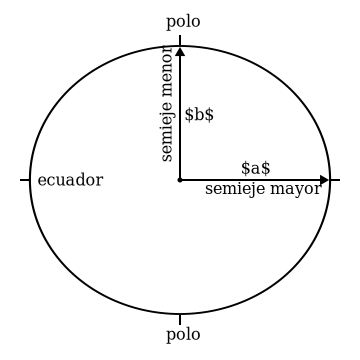
\includegraphics[width=0.7\textwidth]{capitulos/3/figuras/figura1.jpg}
	\caption{\label{fig:intrusiva} Típicas configuraciones de detección intrusiva}	
	%TODO cambiar el texto 3 del gráfico por Detectortes de inducción %
\end{figure}

Un segundo tipo de unidades utiliza \emph{tubos neumáticos} que son extendidos a través de la calzada y que se fijan en la acera en ambos extremos. Una ráfaga de presión de aire se produce en el tubo de goma cuando un vehículo pasa por encima. El pulso de presión de aire cierra un interruptor produciendo una señal eléctrica que es transmitida.

El tercer tipo son los \emph{detectores de bucle de inducción}, que consisten en rollos de alambre recubierto, enterrados en ranuras cortadas en la superficie de la carretera y sellados con masilla. Los datos son enviados a través de un cable enterrado con los bucles hasta una unidad de procesamiento. Una señal eléctrica es aplicada al bucle, la cual oscila en presencia de un vehículo en movimiento. Estos cambios son detectados por la unidad de procesamiento que genera un evento que es transmitido.

Otro tipo de detector intrusivo, denominado \emph{weigh-in-motion} mostrado en la \Cref{fig:Weight-In-Motion}, consisten en un sensor piezoeléctrico ubicado en un canal a través del camino. El sistema registra la variación de tensión medida en los piezoeléctricos, lo cual genera un evento que es transmitido para su procesamiento. Estos sistemas  se utilizan en ubicaciones específicas mayormente para el control de acceso.

\begin{figure}[h]
	\centering
	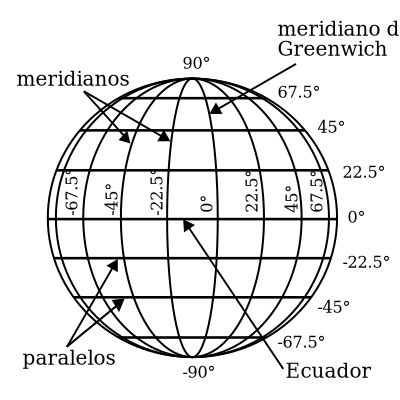
\includegraphics[width=0.7\textwidth]{capitulos/3/figuras/figura2.jpg}
	\caption{\label{fig:Weight-In-Motion}  Sistema de detección weight-in-motion}	
\end{figure}

\subsection{Sensores de tecnología no intrusiva}

Los sensores de tecnología no intrusiva incluyen:  recolección de datos por video, detectores infrarrojos pasivos o activos, radares de microondas, detectores ultrasónicos, detectores acústicos, detectores láser y fotografía aérea. La mayoría de los sistemas no intrusivos son operacional y visualmente similares, consistiendo en pequeñas unidades electrónicas montadas en contenedores a prueba de agua.

\begin{figure}[h]
	\centering
	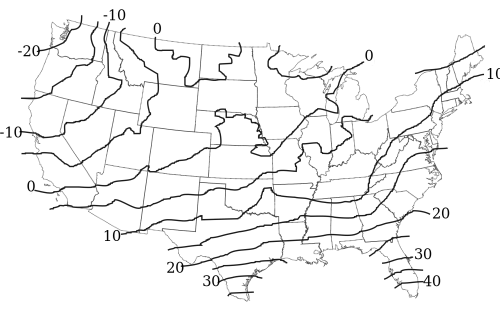
\includegraphics[width=0.7\textwidth]{capitulos/3/figuras/figura3.jpg}
	\caption{\label{fig:noIntrusica}  Configuraciones típicas de tecnologías no intrusivas}	
\end{figure}

En la \Cref{fig:noIntrusica} pueden notarse una disposición de 3 tipos de deterctores no intrusivos. El primer tipo corresponde a los \emph{montados en mástil} al costado de la carretera, tales como cámaras fotográficas o de video, capaces de procesar un campo de visión que cubre un área oblicua, ya sea por encima o por debajo de la unidad.  Problemas de oscurecimiento pueden ocurrir cuando vehículos grandes cubren a vehículos pequeños del detector o cuando el campo de visión es muy grande, causando la detección de vehículos fuera del carril deseado.

El segundo tipo de detectores no son los \emph{montados debajo de puentes o portales}, con un campo de visión justo por debajo de los mismos, o ligeramente oblicuo a la unidad. Este tipo de detectores también está sujeto a los problemas de oscurecimiento mencionados anteriormente.

Finalmente, el tercer tipo, conocidos como de \emph{fuego cruzado}, consiste en unidades tales como monitores de polución que son montados a nivel del piso a ambos lados del camino, disparando un haz a través de la carretera. Estas unidades están sujetas al enmascaramiento de lado a lado, por lo tanto, son más adecuadas para un solo carril.

\section{Tecnologías de Floating Car Data}

Además de la utilización de tecnologías in-situ, muchas aplicaciones de gestión de tráfico utilizan dispositivos montados en vehículos en circulación, conocidos como sistemas de ubicación automática de vehículo (\emph{Automatic Vehicle Location} - AVL). Los dispositivos AVL pueden proveer dos tipos de información: \begin{enumerate*}[a)]
\item información de posición, cuando un vehículo equipado con ellos pasa cierto punto de la red donde existe un sensor, o \item información continua, a medida que el vehículo transita a través de la red.
\end{enumerate*}

Los primeros sistemas AVL se basaron en vehículos equipados con transpondedores que transmitían y recibían información de los dispositivos ubicados en la carretera. Los sistemas actuales se basan en la tecnología del Sistema de Posicionamiento Global (\emph{Global Positioning Systen} - GPS) o en otros mecanismos de posicionamiento para luego transmitir la posición del vehículo.

El principio de FCD es recolectar datos de tráfico en tiempo real ubicando los vehículos a través de dispositivos AVL en toda la red de caminos como se muestra en la \Cref{fig:ComunicacionGPS}. Todos los vehículos equipados con estos dispositivos actúan como sensores dentro de la red de caminos. Datos como la ubicación del vehículo, la velocidad y dirección del viaje son enviados a un centro de procesamiento para la recolección y extracción de información. Luego de la recolección y extracción, información útil como el estado del tráfico y rutas alternativas pueden ser derivadas y posteriormente distribuidas.

\begin{figure}[h]
	\centering
	\includegraphics[width=0.7\textwidth]{capitulos/3/figuras/figura4.jpg}
	\caption{\label{fig:ComunicacionGPS}  Comunicación con GPS}	
\end{figure}

\subsection{FCD basado en GPS}

% Actualmente existen dispositivo AVL que cuentan con sensores GPS. 

Hoy en día la tecnología GPS se encuentra altamente disponible, lo que se refleja en el aumento del número de vehículos y dispositivos móviles equipados con este sistema de ubicación. Esto lleva al desarrollo de trabajos que aprovechan esta tecnología para la obtención de FCD \cite{giovannini2011novel,li2007practical,sevlian2010travel,yin2004weight}

% Esta tecnología permite obtener la ubicación con una precisión relativamente alta, típicamente menor a 30 metros. Generalmente, los datos del tráfico que se obtienen de vehículos privados o camiones con tecnología GPS son más adecuados para autopistas y zonas rurales.

A pesar de la existencia de sistemas FCD que utilizan vehículos sonda equipados con dispositivos AVL basados en GPS \cite{simmons2002commercial,leduc2008road}, que son utilizados como fuente de información en tiempo real. Su aplicación está restringida a un limitado número de vehículos debido a los costos del equipamiento dedicado requerido. 

En comparación, estrategias FCD basadas en dispositivos no dedicados, tales como teléfonos celulares u otros dispositivos móviles, que evitan los costos de equipamiento, son una alternativa que actualmente está recibiendo especial atención \cite{thiagarajan2010cooperative,thiagarajan2009vtrack,de2008traffic}.

\subsection{FCD basado en dispositivos móviles}

La rápida expansión de los teléfonos y dispositivos inteligentes y los múltiples sensores que poseen los mismos, los convierte en una potencial fuente para implementación de sistemas FCD. Muchos trabajos se centran en la utilización de dispositivos móviles para la detección del tráfico, la mayoría aprovechando los sistemas A-GPS\footnote{http://es.wikipedia.org/wiki/GPS\_Asistido}, pero también existen otros que utilizan las redes GSM\footnote{http://en.wikipedia.org/wiki/GSM}, WiFi\footnote{http://en.wikipedia.org/wiki/Wi-Fi} y hasta la tecnología Bluetooth\footnote{http://en.wikipedia.org/wiki/Bluetooth} \cite{thiagarajan2010cooperative,thiagarajan2009vtrack,fraser2007use,fang2011enacq,ruppe2012augmenting}.

En 2007, Fraser \cite{fraser2007use} habla de la viabilidad de utilización de dispositivos móviles como alternativa a los métodos típicos de detección de tráfico, utilizando ubicación de objetos mediante triangulación con antenas de telefonía, tal como se muestra en la \Cref{fig:triangulacionAntenas}. En el mismo trabajo se comenta de las dificultades que tienen tales sistemas en cuanto a la precisión de ubicación, quedando este punto como una problemática a ser resuelta.

\begin{figure}[h]
	\centering
	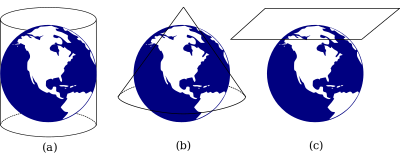
\includegraphics[width=0.7\textwidth]{capitulos/3/figuras/figura5.jpg}
	\caption{\label{fig:triangulacionAntenas} Triangulación de Antenas}	
\end{figure}

A pesar de la baja precisión de los sistemas GSM para la ubicación de dispositivos móviles, se han realizado trabajos como CTrack \cite{thiagarajan2011accurate} que utilizan este método. CTrack utiliza la red GSM y  otros sensores disponibles en el teléfono, tales como el  acelerómetro para detectar movimiento y los compases magnéticos para detectar giros. El sistema consiste en dos componentes de software, una librería para el teléfono y un servicio web. La librería recolecta, filtra y escanea los datos obtenidos con el teléfono y los transmite a través de la red inalámbrica al servicio web, el cual corre un algoritmo de MM sobre los datos recibidos. El trabajo comentado tiene como premisa hacer un uso eficiente del consumo de la batería del dispositivo, evitando usar sensores de alto consumo tales como el sensor GPS o la antena WiFi.

Otro trabajo que busca un uso eficiente de energía es EnAcq \cite{fang2011enacq}. El mismo propone un método de adquisición de ubicaciones y luego realiza un proceso de MM mejorado que se centra en dos desafíos claves: datos imprecisos de trayectoria y consumo eficiente de energía. Para evitar el consumo innecesario de energía, utiliza una estrategia adaptativa para la toma de ubicaciones por GPS, que se basa en el estado de movimiento actual del dispositivo.

También existen trabajos que utilizan otros métodos para detectar la ubicación de los vehículos como la tecnología Bluetooth y las redes WiFi \cite{ruppe2012augmenting}, donde se ven enfoques de bajo coste y gran escala para monitorear el tráfico, que aumentan el principio de FCD y permiten la detección de vehículos, transeúntes, ciclistas y pasajeros del transporte público para lograr datos espacio-temporales de tráfico. Este enfoque se basa en la ubicación indirecta de los objetos sensibles de tráfico (autos, ciclistas. transeúntes) que poseen el WiFi o bluetooth activado por medio de sensores fijos y móviles que constituyen una infraestructura dedicada. Por ejemplo, un auto que está equipado con receptores específicos, detecta todos los objetos de tráfico que están dentro de un área a través del número de identificación de WiFi o Bluetooth, actuando como sensor móvil. Los datos medidos son procesados para obtener las trayectorias, tiempo de viaje, estado del tráfico, matrices de origen-destino y otros parámetros de tráfico.
